\documentclass[handout, 10pt]{beamer}

%\usepackage[backend=bibtex,firstinits=true,style=verbose-inote,citestyle=authortitle]{biblatex}
\usepackage{bm}
\usepackage{graphicx}
\usepackage{subcaption}
\usepackage{amsmath}
\usepackage{amsfonts}
\usepackage{makecell}
\usepackage{filecontents}
\usepackage{biblatex}
\usepackage{xcolor}
\usepackage{subcaption}
 \newcommand{\expect}[2][]{
\ifthenelse{\equal{#1}{}}{
\mathbb{E}\left[#2\right]
}{
\underset{#1}{\mathbb{E}}\left[#2\right]
}}

\newcommand{\cov}[2][]{
\ifthenelse{\equal{#1}{}}{
\text{Cov}\left[#2\right]
}{
\underset{#1}{\text{Cov}}\left[#2\right]
}}


\newcommand{\var}[2][]{
\ifthenelse{\equal{#1}{}}{
\text{Var}[#2]
}{
\underset{#1}{\text{Var}}[#2]
}}

\newcommand{\loss}[2][]{
\ifthenelse{\equal{#1}{}}{
\mathcal{L}(#2)
}{
\mathcal{L}_{#1}(#2)
}}

\newcommand{\kl}[2]{
\text{D}_\text{KL}[#1 \parallel #2]
}

\newcommand{\R}{\mathbb{R}}
%\newcommand{\Prob}{\mathbb{P}}

\newcommand{\1}[1]{\mathds{1}\{#1\}}


%\usecolortheme{dolphin}
\setbeamertemplate{navigation symbols}{}
\setbeamertemplate{section in toc}{\inserttocsectionnumber.~\inserttocsection}

\begin{filecontents*}{references.bib}
@misc{diff_augment,
    title={Differentiable Augmentation for Data-Efficient GAN Training},
    author={Shengyu Zhao and Zhijian Liu and Ji Lin and Jun-Yan Zhu and Song Han},
    year={2020},
    eprint={2006.10738},
    archivePrefix={arXiv},
    primaryClass={cs.CV}
}
\end{filecontents*}

\addbibresource{references.bib}


\title{Differentiable Augmentation for Data-Efficient GAN Training\footnote{\citepaper{diff_augment}}}
%\subtitle{}
%\author{Ivan Skorokhodov}
%\date{}
%\logo{\includegraphics[height=1cm]{images/ipavlov-logo.png}}

\newcommand{\citepaper}[1]{\citetitle{#1} by \citeauthor{#1}, \citeyear{#1}}

%\graphicspath{{./images}}

%\usetheme{lucid}
\begin{document}

\begin{frame}
    \titlepage
\end{frame}

\begin{frame}{Overview}
\begin{itemize}
    \item\pause Training GANs generally requires a lot of data
    \item\pause That's because it is too easy for D to memorize a small training set
    \item\pause When D memorizes the training set, the training dynamics gets disrupted
    \item\pause To alleviate this, people use augmentations
    \begin{itemize}
        \item\pause for reals
        \item\pause for reals and fakes for $D$ only
        \item\pause for reals and fakes for both $D$ and $G$
    \end{itemize}
    \item\pause Authors propose to backprop through augmentations of $G(z)$ and show that it works the best
\end{itemize}
\end{frame}

\begin{frame}{Training without augmentations}
\begin{equation}
\begin{array}{l}
L_{D}=\mathbb{E}_{\boldsymbol{x} \sim p_{\text {data }}(\boldsymbol{x})}\left[f_{D}(-D(\boldsymbol{x}))\right]+\mathbb{E}_{\boldsymbol{z} \sim p(\boldsymbol{z})}\left[f_{D}(D(G(\boldsymbol{z})))\right], \\
L_{G}=\mathbb{E}_{\boldsymbol{z} \sim p(\boldsymbol{z})}\left[f_{G}(-D(G(\boldsymbol{z})))\right]
\end{array}
\end{equation}

\begin{figure}
\centering
\includegraphics[width=\textwidth]{images/training-without-augs}
\end{figure}
\end{frame}


\begin{frame}{Augmenting only reals}
\begin{equation}
\begin{array}{l}
L_{D}=\mathbb{E}_{\boldsymbol{x} \sim p_{\text {data }}(\boldsymbol{x})}\left[f_{D}(-D(\textcolor{red}{T}(\boldsymbol{x})))\right]+\mathbb{E}_{\boldsymbol{z} \sim p(\boldsymbol{z})}\left[f_{D}(D(G(\boldsymbol{z})))\right], \\
L_{G}=\mathbb{E}_{\boldsymbol{z} \sim p(\boldsymbol{z})}\left[f_{G}(-D(G(\boldsymbol{z})))\right]
\end{array}
\end{equation}

\begin{figure}
\centering
\includegraphics[width=0.5\textwidth]{images/aug-reals-only}
\end{figure}
\textbf{Main problem}: $G$ starts producing augmentations as well (cutouts, color jitters, etc)
\end{frame}


\begin{frame}{Augmenting only $D$}
\begin{equation}
\begin{array}{l}
L_{D}=\mathbb{E}_{\boldsymbol{x} \sim p_{\text {data }}(\boldsymbol{x})}\left[f_{D}(-D(\textcolor{red}{T}(\boldsymbol{x})))\right]+\mathbb{E}_{\boldsymbol{z} \sim p(\boldsymbol{z})}\left[f_{D}(D(\textcolor{red}{T}(G(\boldsymbol{z}))))\right], \\
L_{G}=\mathbb{E}_{\boldsymbol{z} \sim p(\boldsymbol{z})}\left[f_{G}(-D(G(\boldsymbol{z})))\right]
\end{array}
\end{equation}

\begin{figure}
\centering
\includegraphics[width=0.5\textwidth]{images/aug-d-only.png}
\end{figure}
\textbf{Main problem}: it becomes too easy for $G$ to fool $D$:
\begin{figure}
    \item\pause $D$ recognizes reals well, but fakes very badly
\end{figure}
\end{frame}


\begin{frame}{Using DiffAug decreases train accuracy and improves val accuracy}
\begin{equation}
\begin{array}{l}
L_{D}=\mathbb{E}_{\boldsymbol{x} \sim p_{\text {data }}(\boldsymbol{x})}\left[f_{D}(-D(\textcolor{red}{T}(\boldsymbol{x})))\right]+\mathbb{E}_{\boldsymbol{z} \sim p(\boldsymbol{z})}\left[f_{D}(D(\textcolor{red}{T}(G(\boldsymbol{z}))))\right], \\
L_{G}=\mathbb{E}_{\boldsymbol{z} \sim p(\boldsymbol{z})}\left[f_{G}(-D(\textcolor{red}{T}(G(\boldsymbol{z}))))\right]
\end{array}
\end{equation}

\begin{figure}
\centering
\includegraphics[width=\textwidth]{images/diffaug-different-types}
\end{figure}
Core idea: to augment fakes \textit{our augmentations must be differentiable}.
\end{frame}


\begin{frame}{Quantitive results on CIFAR-10 on 100\% data}
\begin{figure}
\centering
\includegraphics[width=\textwidth]{images/cifar10-comparison-table}
\end{figure}
\end{frame}


\begin{frame}{Quantitative results on limited data}
\begin{figure}
\centering
\includegraphics[width=\textwidth]{images/diffaug-vs-stylegan2-limited-data-results}
\end{figure}
\begin{figure}
\centering
\includegraphics[width=\textwidth]{images/diffaug-vs-pretrained-models-limited-data-results}
\end{figure}
\end{frame}


\begin{frame}{Qualitative results on limited data}
\begin{figure}
\centering
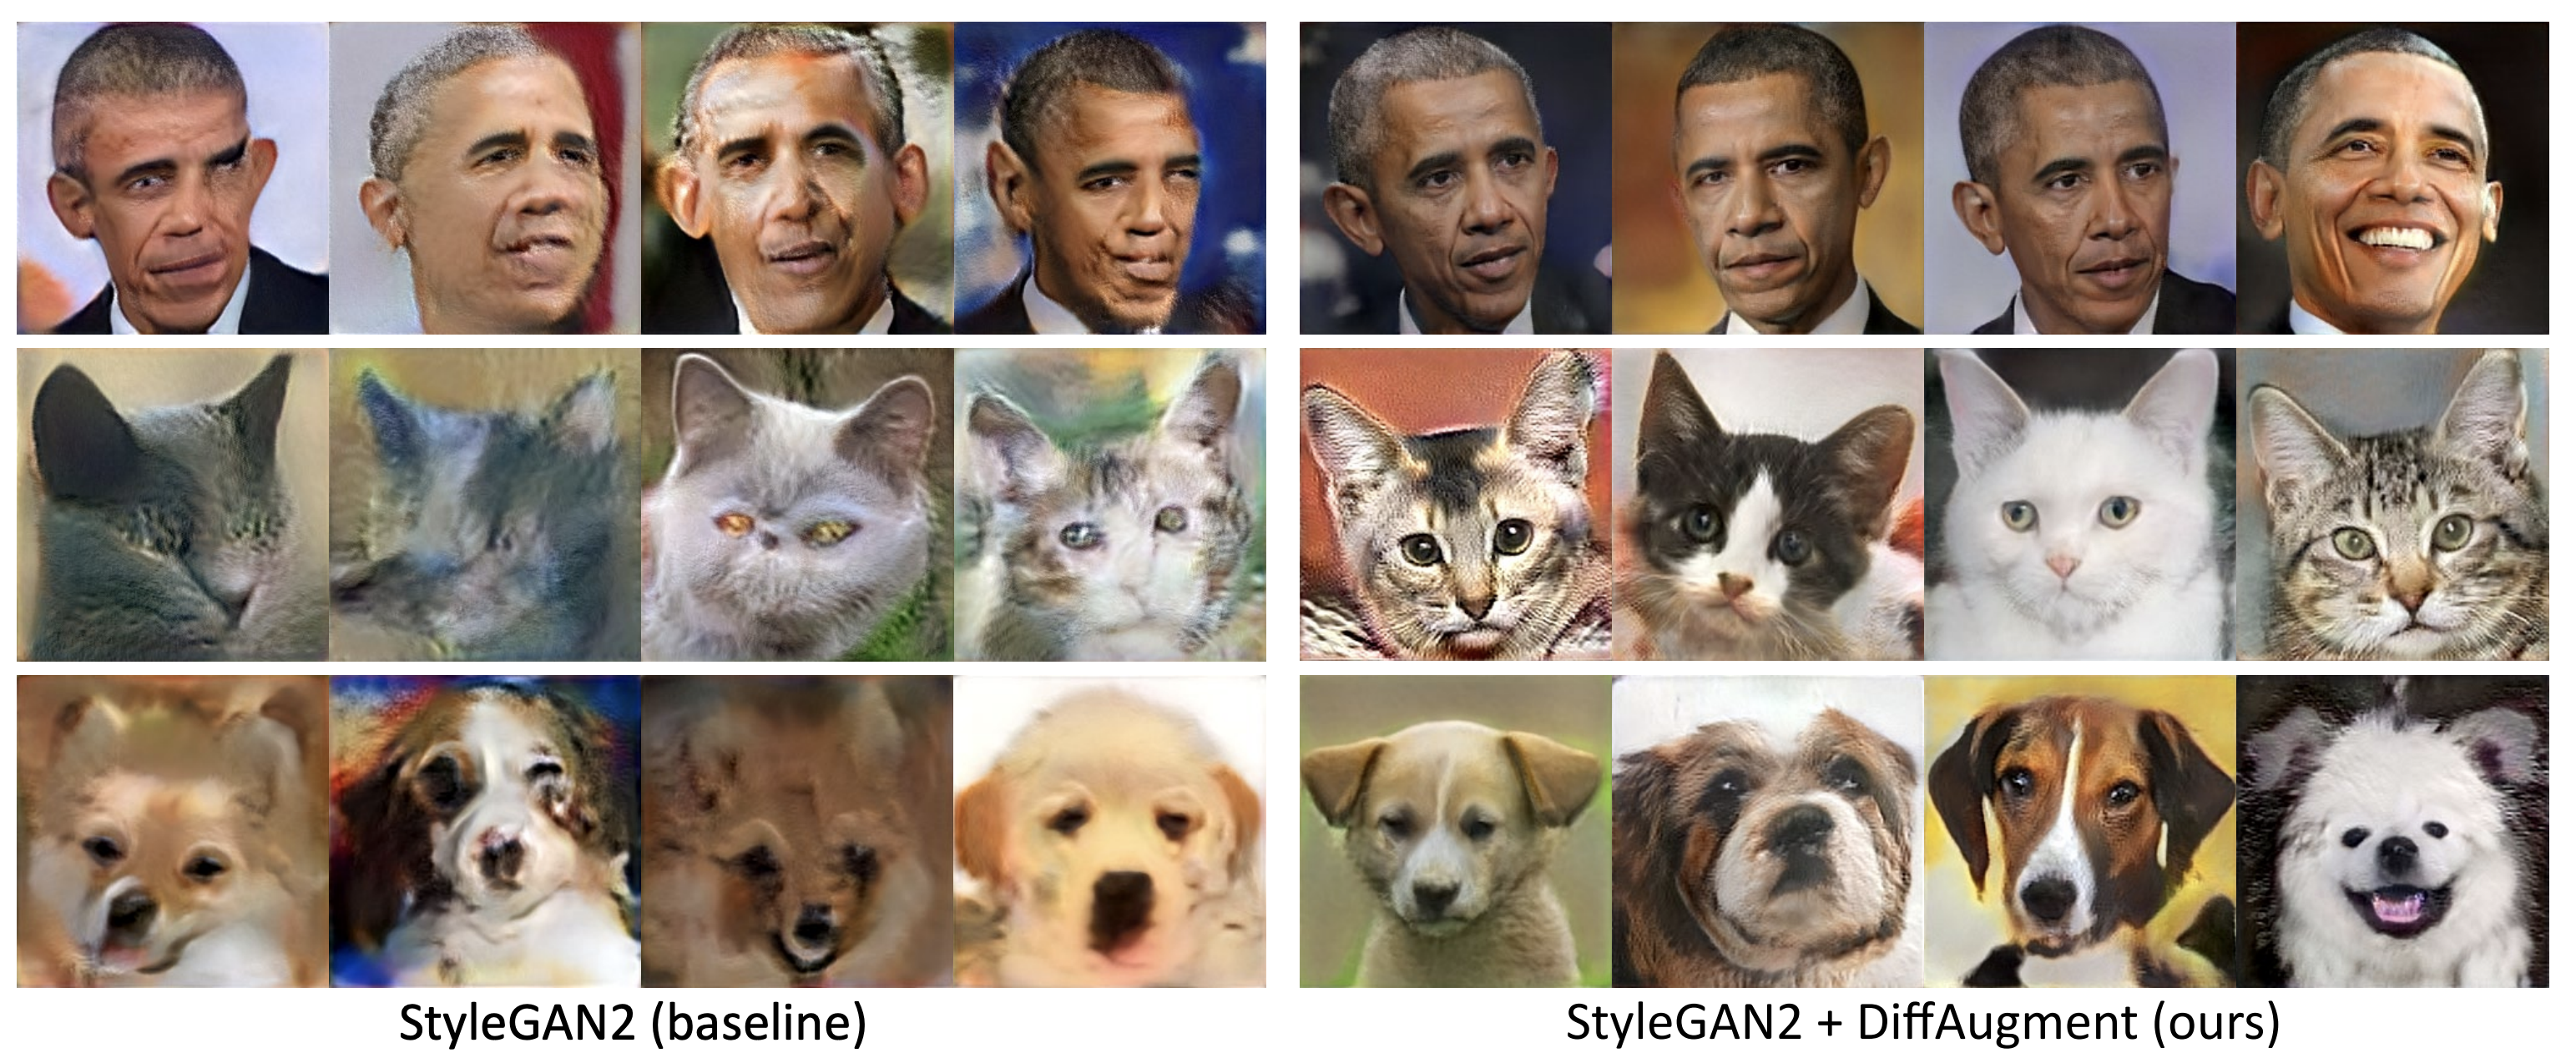
\includegraphics[width=\textwidth]{images/diffaugs-vs-stylegan2-samples}
\caption{Few-shot generation. Faces: 100-shot, cats: 160-shot, dogs: 389-shot. Resolution: $256 \times 256$}
\end{figure}
\end{frame}


\begin{frame}{Final thoughts}
\begin{itemize}
    \item\pause DiffAugs are easy to implement and they are fast.
    \item\pause Self-supervised learning is very simple to incorporate and boosts scores in many areas
    \begin{itemize}
        \item\pause Where else can we apply it?
    \end{itemize}
    \item\pause Next step: more powerful augmentations? FixMatch/SimCLR/etc have much more augmentations under the hood.
    \item\pause Next step: parametrized differentiable augmentations?
    \begin{itemize}
        \item\pause It will be very similar to Spatial Transformer Networks then
    \end{itemize}
\end{itemize}
\end{frame}

\end{document}
